\documentclass[10pt,a4paper,fleqn]{article}
\usepackage[utf8]{inputenc}
\usepackage[portuguese]{babel}
\usepackage[T1]{fontenc}
\usepackage{amsmath}
\usepackage{amsfonts}
\usepackage{amssymb}
\usepackage{graphicx}
\usepackage{setspace}
\usepackage{enumerate}

\title{Disciplina M\'{e}todos Potenciais}
\author{Vanderlei C. Oliveira Jr.}
\date{}

\doublespace

\begin{document}

\begin{center}

\begin{huge}
\emph{Representação dos campos de gravidade e geomagnético em Harmônicos Esféricos}
\end{huge}

\bigskip
\bigskip

\begin{large}
\emph{Disciplina M\'{e}todos Potenciais}
\end{large}

\end{center}

\bigskip
\bigskip

\begin{center}

\fbox{\begin{minipage}{15em}

\begin{center}

Vanderlei C. Oliveira Jr.

Observat\'{o}rio Nacional

Rio de Janeiro - 2020

\end{center}

\end{minipage}}

\end{center}

\clearpage

\tableofcontents

\clearpage

%%%%%%%%%%%%%% Harmônicos esféricos %%%%%%%%%%%%%%
%%%%%%%%%%%%%%%%%%%%%%%%%%%%%%%%%%%%%%%%%%%%%%%%%%
\part{Harm\^{o}nicos esf\'{e}ricos}

%%%%% Exercício 2.1 %%%%%
\section{Equa\c{c}\~{o}es diferenciais auxiliares}

\subsection{Equa\c{c}\~{o}es de $r$}

Sejam $f_{1}(r)$ e $f_{2}(r)$ duas fun\c{c}\~{o}es dadas por
\begin{equation}
f_{1}(r) = r^{n}
\label{eq:ex211-r^}
\end{equation}
e
\begin{equation}
f_{2}(r) = r^{-(n+1)} \quad ,
\label{eq:ex211-r_}
\end{equation}
em que $n \geqslant 0$ \'{e} um n\'{u}mero inteiro e $r > 0$ \'{e} um n\'{u}mero real. 

\begin{flushleft}
\dotfill
\end{flushleft}

\subsubsection{Exerc\'{i}cio}

Mostre que $f_{1}(r)$ (Eq. \ref{eq:ex211-r^}) e $f_{2}(r)$ (Eq. \ref{eq:ex211-r_}) 
s\~{a}o solu\c{c}\~{o}es da equa\c{c}\~{a}o diferencial
\begin{equation}
r^{2} \: \frac{d^{2} f(r)}{d r^{2}} + 2 \: r \: \frac{d \, f(r)}{d r} - n(n+1) \: f(r) = 0 \quad .
\label{eq:ex211-eqdif-r}
\end{equation}

\begin{flushleft}
\dotfill
\end{flushleft}

%%%%% Exercício 2.2 %%%%%
\subsection{Equa\c{c}\~{o}es de $\lambda$}

Sejam $h_{1}(\lambda)$ e $h_{2}(\lambda)$ duas fun\c{c}\~{o}es dadas por
\begin{equation}
h_{1}(\lambda) = \text{cos}(m \lambda)
\label{eq:ex212-cos}
\end{equation}
e
\begin{equation}
h_{2}(\lambda) = \text{sen}(m \lambda) \quad ,
\label{eq:ex212-sen}
\end{equation}
em que $m \geqslant 0$ \'{e} um n\'{u}mero inteiro e $\lambda$ \'{e} um n\'{u}mero real. 

\begin{flushleft}
\dotfill
\end{flushleft}

\subsubsection{Exerc\'{i}cio}

Mostre que
$h_{1}(\lambda)$ (Eq. \ref{eq:ex212-cos}) e $h_{2}(\lambda)$ (Eq. \ref{eq:ex212-sen}) 
s\~{a}o solu\c{c}\~{o}es da equa\c{c}\~{a}o diferencial
\begin{equation}
\frac{d^{2} h(\lambda)}{d \lambda^{2}} + m^{2} h(\lambda) = 0 \quad .
\label{eq:ex212-eqdif-lamb}
\end{equation}

\begin{flushleft}
\dotfill
\end{flushleft}

%%%%% Exercício 2.3 %%%%%
\subsection{Polin\^{o}mios de Legendre}

A equa\c{c}\~{a}o diferencial
\begin{equation}
\text{sen} \theta \, g''(\theta) + 
\text{cos} \theta \, g'(\theta) + 
\left[ n(n+1) \, \text{sen} \theta - \dfrac{m^{2}}{\text{sen} \theta} \right] = 0
\label{eq:ex213-eq-diff-Legendre-theta}
\end{equation}
tem como solu\c{c}\~{a}o os \textit{Polin\^{o}mios associados de Legendre}
\begin{equation}
g(\theta) = P_{nm}(\text{cos}\theta) \quad .
\label{eq:ex213-g-theta}
\end{equation}
Nestas Equa\c{c}\~{o}es, $n$ e $m$ s\~{a}o inteiros maiores ou iguais a zero (sendo $m$ menor ou igual a $n$), 
$g'(\theta)$ \'{e} a primeira derivada e $g''(\theta)$ \'{e} a segunda derivada de $g(\theta)$. Os inteiros $n$ 
e $m$ s\~{a}o, respectivamente, o grau e a ordem do polin\^{o}mio $P_{nm}(\text{cos}\theta)$. Por conveni\^{e}ncia, 
estas Equa\c{c}\~{o}es s\~{a}o comumente transformadas por mudan\c{c}a de vari\'{a}veis  utilizando a rela\c{c}\~{a}o 
$t = \text{cos}(\theta)$. Dessa forma,
\begin{equation}
\begin{array}{l}
g(\theta) = \overline{g}(t) \\
g'(\theta) = -\overline{g}'(t) \, \text{sen} \theta \\
g''(\theta) = \overline{g}''(t) \, \text{sen}^{2} \theta - \overline{g}'(t) \, \text{cos} \theta \quad .
\end{array}
\label{eq:ex213-g-t}
\end{equation}
em que $\overline{g}(t) = P_{nm}(t)$, com primeira e segunda derivadas $\overline{g}'(t)$ e $\overline{g}''(t)$, 
respectivamente. Substituindo as Equa\c{c}\~{o}es \ref{eq:ex213-g-t} na equa\c{c}\~{a}o diferencial 
\ref{eq:ex213-eq-diff-Legendre-theta}, dividindo o resultado por $\text{sen} \theta$ e utilizando a rela\c{c}\~{a}o $\text{sen}^{2} 
\theta = 1 - t^2$ temos que
\begin{equation}
(1 - t^2) \, \overline{g}''(t) - 2 \, t \, \overline{g}'(t) +
\left[ n(n+1) - \frac{m^{2}}{1 - t^2} \right] = 0 \quad .
\label{eq:ex213-eq-diff-Legendre-t}
\end{equation}
A fun\c{c}\~{a}o $\overline{g}(t) = P_{nm}(t)$ (polin\^{o}mio associado de Legendre escrito em fun\c{c}\~{a}o da viari\'{a}vel 
$t$) que satisfaz a Equa\c{c}\~{a}o \ref{eq:ex213-eq-diff-Legendre-t} pode ser dada por
\begin{equation}
P_{nm}(t) = \frac{1}{2^{n} \, n!} \, (1 - t^{2})^{m/2} \,
\frac{d^{n+m}}{d \, t^{n+m}}(t^{2} - 1)^{n} \quad .
\label{eq:ex213-pnm-t}
\end{equation}
Por exemplo,
\begin{equation}
\begin{split}
P_{11}(t) & = \frac{(1 - t^{2})^{1/2}}{2} \, \frac{d^{2}}{d \, t^{2}}(t^{2} - 1) \\
& = \sqrt{1 - t^{2}} \\
& = \text{sen} \theta \quad ,
\end{split}
\label{eq:ex213-p11-t}
\end{equation}
ou
\begin{equation}
\begin{split}
P_{21}(t) & = \frac{(1 - t^{2})^{1/2}}{2^{2} \, 2!} \, \frac{d^{3}}{d \, t^{3}}(t^{2} - 1)^{2} \\
& = \frac{\sqrt{1 - t^{2}}}{8} \, (16 \, t + 8 \, t) \\
& = 3 \, t \, \sqrt{1 - t^{2}} \\
& = 3 \, \text{sen} \theta \, \text{cos} \theta \quad .
\end{split}
\label{eq:ex213-p21-t}
\end{equation}
No caso particular em que $m = 0$, n\~{a}o h\'{a} ra\'{i}zes $\sqrt{1 - t^{2}}$, $P_{nm}(t)$ \'{e} representado 
simplesmente por $P_{n}(t)$ e \'{e} denominado \textit{Polin\^{o}mio de Legendre}. A partir da Equa\c{c}ão \ref{eq:ex213-pnm-t}, 
os polin\^{o}mios de Legendre podem ser escritos como
\begin{equation}
P_{n}(t) = \frac{1}{2^{n} \, n!} \frac{d^{n}}{d \, t^{n}}(t^{2} - 1)^{n} \quad .
\label{eq:ex213-pn-t}
\end{equation}
Alternativamente, os polin\^{o}mios de Legendre (\ref{eq:ex213-pn-t}) a partir do grau $n = 2$ podem ser obtidos pela 
f\'{o}rmula recursiva
\begin{equation}
P_{n}(t) = - \, \frac{n - 1}{n} \, P_{n-2}(t) + \frac{2n - 1}{n} \, t \, P_{n-1}(t) \quad ,
\label{eq:ex213-pn-recursiva}
\end{equation}
em que $P_{2}(t)$ \'{e} obtido utilizando $P_{0}(t)$ e $P_{1}(t)$, $P_{3}(t)$ \'{e} obtido utilizando $P_{1}(t)$ e $P_{2}(t)$, etc.

\begin{flushleft}
\dotfill
\end{flushleft}

\subsubsection{Exerc\'{i}cio}

Determine:
\begin{enumerate}[(i)]

\item os polin\^{o}mios associados de Legendre de grau $n = 0$ e ordem $m = 0$ at\'{e} grau $n = 3$ 
e ordem $m = 3$ utilizando a Equa\c{c}ão \ref{eq:ex213-pnm-t}.

\item os polin\^{o}mios de Legendre de grau $n = 0$ at\'{e} $n = 5$ utilizando a Equa\c{c}ão 
\ref{eq:ex213-pn-t}.

\item os polin\^{o}mios de Legendre de grau $n = 2$ at\'{e} $n = 5$ utilizando a 
f\'{o}rmula recursiva representada pela Equa\c{c}\~{a}o \ref{eq:ex213-pn-recursiva}.

\end{enumerate}

\subsubsection{Exerc\'{i}cio}

Fa\c{c}a um gr\'{a}fico dos polin\^{o}mios de Legendre $P_{n}(t)$ de grau 
$n = 0$ at\'{e} $n = 5$ para $t$ no intervalo $[-1,1]$. 

\begin{flushleft}
\dotfill
\end{flushleft}

%%%%% Exercício 2.4 %%%%%
\section{Equa\c{c}\~{a}o de Laplace em coordenadas esf\'{e}ricas}

Seja $V(r,\theta,\lambda)$ uma fun\c{c}\~{a}o harm\^{o}nica que depende das coordenadas esf\'{e}ricas $r$, $\theta$ e $\lambda$ 
(Fig. \ref{fig:fig2}). Esta fun\c{c}\~{a}o satisfaz a equa\c{c}\~{a}o de Laplace em coordenadas esf\'{e}ricas, que pode ser escrita como
\begin{equation}
r^{2} \, \frac{\partial^{2} \, V}{\partial \, r^{2}} +
2 \, r \, \frac{\partial \, V}{\partial \, r} +
\frac{\partial^{2} \, V}{\partial \, \theta^{2}} +
\text{cot} \theta \, \frac{\partial \, V}{\partial \, \theta} +
\frac{1}{\text{sen}^{2} \theta} \, \frac{\partial^{2} \, V}{\partial \, \lambda^{2}} = 0 \quad .
\label{eq:ex214-eq-Laplace-esferica}
\end{equation}

%Figuras ==>
\begin{figure}[h]
    \centering
    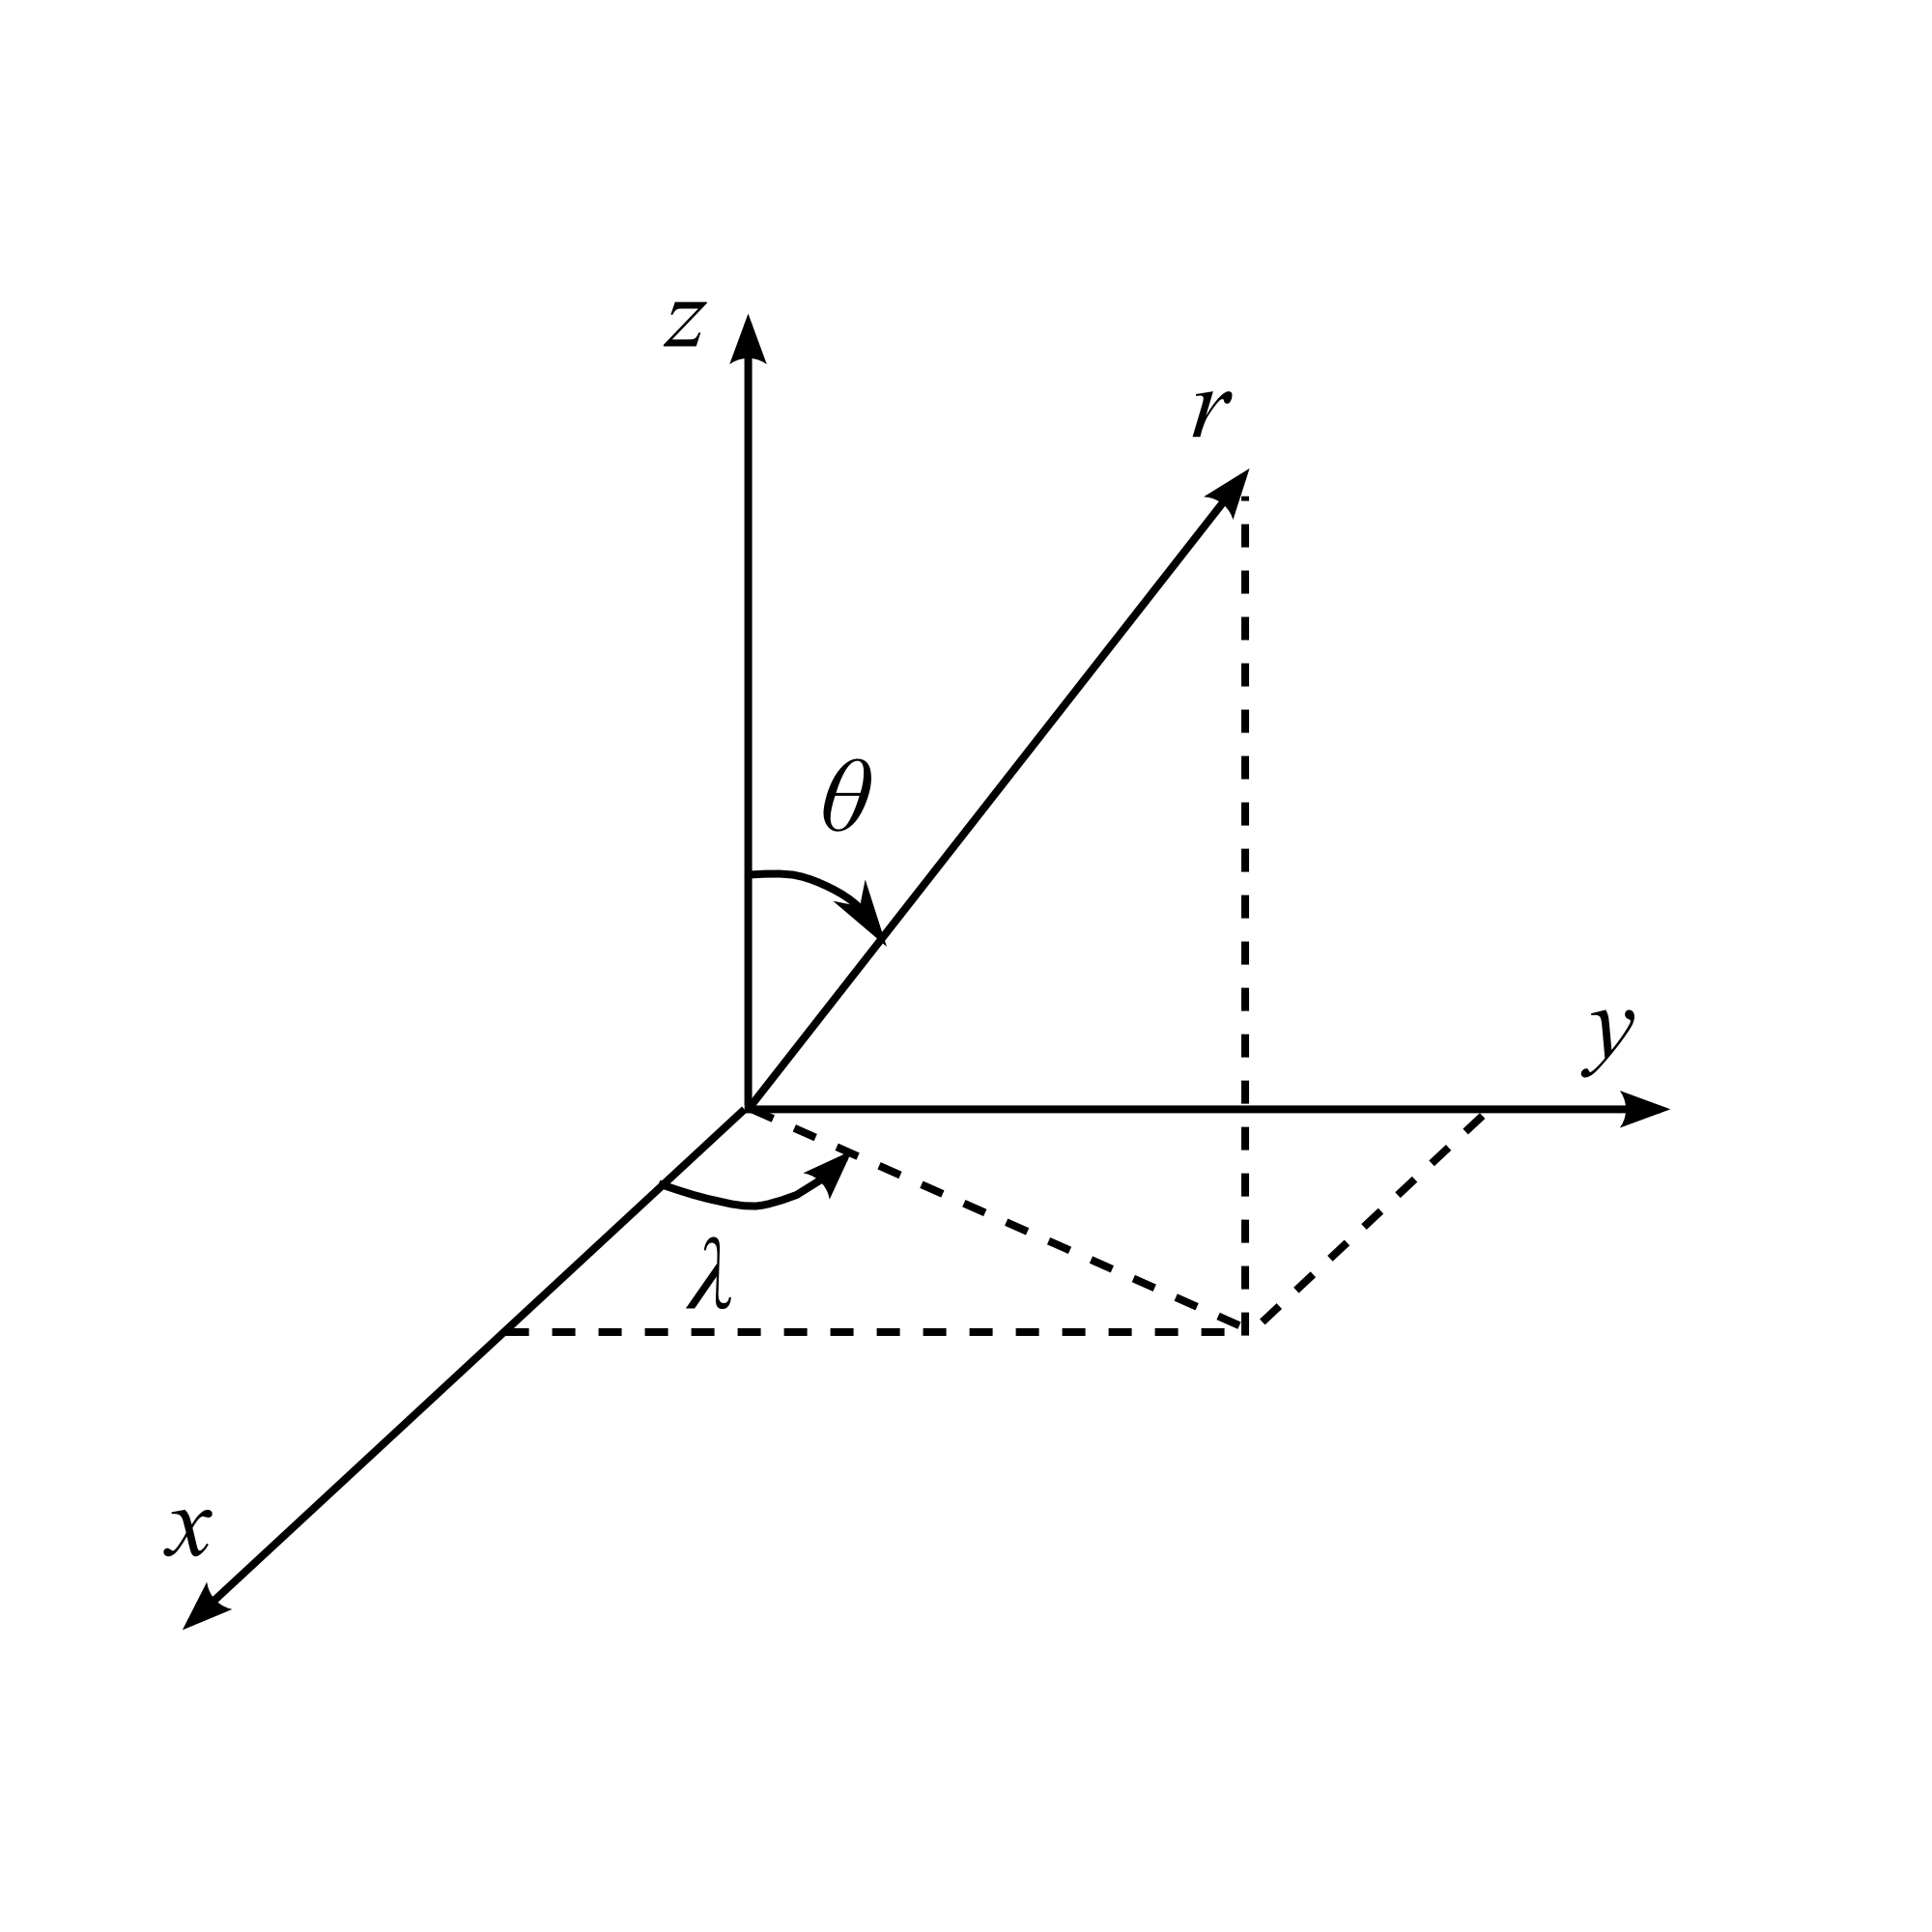
\includegraphics[scale=1]{Fig2.png}
    \caption{Sistema de coordenadas Cartesianas $(x,y,z)$ e esf\'{e}ricas $(r,\theta,\lambda)$.}
    \label{fig:fig2}
\end{figure}
%<== Figuras

\subsection{Solu\c{c}\~{a}o da Equa\c{c}\~{a}o de Laplace em coordenadas esf\'{e}ricas}

A equa\c{c}ão de Laplace \ref{eq:ex214-eq-Laplace-esferica} pode ser resolvida pelo m\'{e}todo de separa\c{c}\~{a}o de vari\'{a}veis. 
Este m\'{e}todo consiste em supor que a fun\c{c}\~{a}o $V(r,\theta,\lambda)$ pode ser reescrita como o produto entre tr\^{e}s fun\c{c}\~{o}es 
independentes:
\begin{equation}
V(r,\theta,\lambda) = f(r) \, g(\theta) \, h(\lambda) \quad .
\label{eq:ex214-v-fhg}
\end{equation}
O pr\'{o}ximo passo consiste em determinar as fun\c{c}\~{o}es $f(r)$, $g(\theta)$ e $h(\lambda)$. Para tanto, basta substituir a fun\c{c}\~{a}o 
$V(r,\theta,\lambda)$ dada pela Equa\c{c}\~{a}o \ref{eq:ex214-v-fhg} na equa\c{c}\~{a}o de Laplace \ref{eq:ex214-eq-Laplace-esferica}. Esta 
substitui\c{c}\~{a}o nos leva a conclus\~{a}o de que a fun\c{c}\~{a}o $f(r)$ (Eq. \ref{eq:ex214-v-fhg}) satisfaz a equa\c{c}\~{a}o diferencial 
\ref{eq:ex211-eqdif-r}. Tal como visto anteriormente, as fun\c{c}\~{o}es $f_{1}(r)$ (Eq. \ref{eq:ex211-r^}) e $f_{2}(r)$ 
(Eq. \ref{eq:ex211-r_}) s\~{a}o solu\c{c}\~{o}es desta equa\c{c}\~{a}o. Neste caso, mostra-se que a fun\c{c}\~{a}o $V(r,\theta,\lambda)$ pode 
ser escrita como:
\begin{equation}
V(r,\theta,\lambda) = r^{n} \, g(\theta) \, h(\lambda) \quad ,
\label{eq:ex214-v-f1gh}
\end{equation}
ou
\begin{equation}
V(r,\theta,\lambda) = \frac{1}{r^{(n+1)}} \, g(\theta) \, h(\lambda) \quad .
\label{eq:ex214-v-f2gh}
\end{equation}
De forma an\'{a}loga, mostra-se que a fun\c{c}\~{a}o 
$h(\lambda)$ (Eq. \ref{eq:ex214-v-fhg}) satisfaz a equa\c{c}\~{a}o diferencial \ref{eq:ex212-eqdif-lamb}, que possui as solu\c{c}\~{o}es 
$h_{1}(\lambda)$ (Eq. \ref{eq:ex212-cos}) e $h_{2}(\lambda)$ (Eq. \ref{eq:ex212-sen}), e que a fun\c{c}\~{a}o $g(\theta)$ (Eq. 
\ref{eq:ex214-v-fhg}) satisfaz a equa\c{c}\~{a}o diferencial \ref{eq:ex213-eq-diff-Legendre-theta}, cuja solu\c{c}\~{a}o \'{e} dada 
pelos polin\^{o}mios associados de Legendre $P_{nm}(\text{cos}\theta)$ (Eq. \ref{eq:ex213-g-theta}). Os polin\^{o}mios associados de 
Legendre $P_{nm}(\text{cos}\theta)$ podem ser obtidos pela Equa\c{c}ão \ref{eq:ex213-pnm-t}, em que $t = \text{cos} \theta$. Por fim, \'{e} poss\'{i}vel 
mostrar que a fun\c{c}\~{a}o $V(r,\theta,\lambda)$ pode ser escrita de duas formas:
\begin{equation}
V_{e}(r,\theta,\lambda) = \sum_{n=0}^{\infty} r^{n} \, 
Y_{n}(\theta, \lambda) \quad ,
\label{eq:ex214-ve}
\end{equation}
ou
\begin{equation}
V_{i}(r,\theta,\lambda) = \sum_{n=0}^{\infty} \frac{1}{r^{(n+1)}} \,
Y_{n}(\theta, \lambda) \quad ,
\label{eq:ex214-vi}
\end{equation}
em que 
\begin{equation}
Y_{n}(\theta, \lambda) = \sum_{m=0}^{n} 
\left[ 
A_{nm} \, R_{nm}(\theta, \lambda) +
B_{nm} \, S_{nm}(\theta, \lambda)
\right] \quad ,
\label{eq:ex214-Yn}
\end{equation}
sendo $A_{nm}$ e $B_{nm}$ constantes e as fun\c{c}\~{o}es $R_{nm}(\theta, \lambda)$ e $S_{nm}(\theta, \lambda)$ dadas por
\begin{equation}
R_{nm}(\theta, \lambda) = P_{nm}(\text{cos}\theta) \, \text{cos}(m \, \lambda)
\label{eq:ex214-rnm}
\end{equation}
e
\begin{equation}
S_{nm}(\theta, \lambda) = P_{nm}(\text{cos}\theta) \, \text{sen}(m \, \lambda) \quad .
\label{eq:ex214-snm}
\end{equation}
As fun\c{c}\~{o}es $V_{e}(r,\theta,\lambda)$ (Eq. \ref{eq:ex214-ve}) e
$V_{i}(r,\theta,\lambda)$ (Eq. \ref{eq:ex214-vi}) s\~{a}o denominadas 
\textit{harm\^{o}nicos esf\'{e}ricos s\'{o}lidos}. Já as fun\c{c}\~{o}es $Y_{n}(\theta, \lambda)$ 
(Eq. \ref{eq:ex214-Yn}) s\~{a}o denominadas \textit{harm\^{o}nicos (esf\'{e}ricos) de superf\'{i}cie}.


\subsection{Rela\c{c}\~{o}es de ortogonalidade entre as fun\c{c}\~{o}es $R_{nm}(\theta, \lambda)$ e $S_{nm}(\theta, \lambda)$}

As expressões analíticas que descrevem as constantes $A_{nm}$ e $B_{nm}$ (Eq. \ref{eq:ex214-Yn}) 
podem ser determinadas por meio das rela\c{c}\~{o}es de ortogonalidade entre as
fun\c{c}\~{o}es $R_{nm}(\theta, \lambda)$ (Eq. \ref{eq:ex214-rnm}) e $S_{nm}(\theta, \lambda)$ 
(Eq. \ref{eq:ex214-snm}). Para tanto, vamos
considerar $r = 1$ nas equa\c{c}\~{o}es \ref{eq:ex214-ve} e \ref{eq:ex214-vi}. Dessa maneira, estas 
equa\c{c}\~{o}es s\~{a}o iguais a uma fun\c{c}\~{a}o 
$f(\theta,\lambda)$ que pode ser escrita em fun\c{c}\~{a}o dos harm\^{o}nicos de superf\'{i}cie 
(Eq. \ref{eq:ex214-Yn}) da seguinte forma
\begin{equation}
\begin{split}
f(\theta,\lambda) & = \sum_{n=0}^{\infty} 
Y_{n}(\theta, \lambda) \\
& = \sum_{n=0}^{\infty} \,
\sum_{m=0}^{n} \left[ 
A_{nm} \, R_{nm}(\theta, \lambda) +
B_{nm} \, S_{nm}(\theta, \lambda)
\right] \: .
\end{split}
\label{eq:ex214-f}
\end{equation}
De acordo com as rela\c{c}\~{o}es de ortogonalidade entre as fun\c{c}\~{o}es $R_{nm}(\theta, \lambda)$ 
(Eq. \ref{eq:ex214-rnm}) e 
$S_{nm}(\theta, \lambda)$ (Eq. \ref{eq:ex214-snm}),
\begin{equation}
\iint \limits_{\sigma}
R_{nm}(\theta, \lambda) \, R_{op}(\theta, \lambda) \, d \sigma  = 0
\label{eq:ex214-ortog-rnm}
\end{equation}
e
\begin{equation}
\iint \limits_{\sigma}
S_{nm}(\theta, \lambda) \, S_{op}(\theta, \lambda) \, d \sigma = 0
\label{eq:ex214-ortog-snm}
\end{equation}
para o caso em que $nm \neq op$. J\'{a} a integral
\begin{equation}
\iint \limits_{\sigma}
R_{nm}(\theta, \lambda) \, S_{op}(\theta, \lambda) \, d \sigma  = 0
\label{eq:ex214-ortog-rnm-snm}
\end{equation}
\'{e} sempre zero, independente dos valores de $o$ e $p$. Nestas Equa\c{c}\~{o}es, 
$\iint \limits_{\sigma} = \int_{\lambda = 0}^{2\pi} \, \int_{\theta = 0}^{\pi}$ e $d 
\sigma = sen\theta \, d\theta d\lambda$. Por outro lado, estas integrais s\~{a}o diferentes 
de zero quando $nm = op$. Neste caso,
\begin{equation}
\iint \limits_{\sigma}
R_{n0}^{2}(\theta, \lambda) \, d \sigma  = \dfrac{4 \, \pi}{2 \, n + 1}
\label{eq:ex214-ortog-rn02}
\end{equation}
e
\begin{equation}
\left.
\begin{array}{l}
\iint \limits_{\sigma}
R_{nm}^{2}(\theta, \lambda) \, d \sigma \\
\iint \limits_{\sigma}
S_{nm}^{2}(\theta, \lambda) \, d \sigma
\end{array}
\right \} =
\dfrac{2 \, \pi}{2 \, n + 1} \dfrac{(n + m)!}{(n - m)!} \: .
\label{eq:ex214-ortog-rnm2-snm2}
\end{equation}
Observe que estas integrais (Eqs. \ref{eq:ex214-ortog-rnm}, \ref{eq:ex214-ortog-snm}, \ref{eq:ex214-ortog-rnm-snm},
\ref{eq:ex214-ortog-rn02} e \ref{eq:ex214-ortog-rnm2-snm2}) s\~{a}o avaliadas sobre a superf\'{i}cie $\sigma$ de uma esfera
com raio unit\'{a}rio, cuja \'{a}rea \'{e} igual a $4 \, \pi$.


\subsection{Determina\c{c}\~{a}o das expressões analíticas que descrevem as constantes $A_{nm}$ e $B_{nm}$}

Para determinar as expressões analíticas que descrevem as constantes $A_{nm}$ (Eqs. \ref{eq:ex214-Yn} e 
\ref{eq:ex214-f}), basta multiplicar os 
dois lados da Equa\c{c}ão \ref{eq:ex214-f} por $R_{op}(\theta,\lambda)$ (Eq. \ref{eq:ex214-rnm}), integrar o resultado sobre 
a superf\'{i}cie $\sigma$ de uma esfera com raio unit\'{a}rio e utilizar as rela\c{c}\~{o}es de ortogonalidade 
(Eqs. \ref{eq:ex214-ortog-rnm}, \ref{eq:ex214-ortog-snm}, \ref{eq:ex214-ortog-rnm-snm}, \ref{eq:ex214-ortog-rn02} e 
\ref{eq:ex214-ortog-rnm2-snm2}):
\begin{equation}
\begin{split}
R_{op}(\theta,\lambda) \, f(\theta,\lambda)
& = R_{op}(\theta,\lambda) \, \sum_{n=0}^{\infty} \,
\sum_{m=0}^{n} \left[ 
A_{nm} \, R_{nm}(\theta, \lambda) +
B_{nm} \, S_{nm}(\theta, \lambda)
\right] \\
& \begin{array}{r} =
\left[ A_{00} \, R_{op}(\theta,\lambda) \, R_{00}(\theta, \lambda) \right. + \\
B_{00} \, R_{op}(\theta,\lambda) \, S_{00}(\theta, \lambda) + \\
A_{10} \, R_{op}(\theta,\lambda) \, R_{10}(\theta, \lambda) + \\
B_{10} \, R_{op}(\theta,\lambda) \, S_{10}(\theta, \lambda) + \\
A_{11} \, R_{op}(\theta,\lambda) \, R_{11}(\theta, \lambda) + \\
B_{11} \, R_{op}(\theta,\lambda) \, S_{11}(\theta, \lambda) + \\
\vdots \quad \quad \quad \quad \quad \\
A_{op} \, R_{op}(\theta,\lambda) \, R_{op}(\theta, \lambda) + \\
B_{op} \, R_{op}(\theta,\lambda) \, S_{op}(\theta, \lambda) + \\
\vdots \quad \quad \quad \quad \quad \\
A_{nn} \, R_{op}(\theta,\lambda) \, R_{nn}(\theta, \lambda) + \\
\left. B_{nn} \, R_{op}(\theta,\lambda) \, S_{nn}(\theta, \lambda) \right]
\end{array} \\
& = \left[ \, \hdots + A_{op} \, R_{op}^{2}(\theta,\lambda) + \hdots \, \right]
\end{split}
\label{eq:ex214-int-Anm-desenvolv}
\end{equation}

\begin{equation}
\begin{split}
\iint \limits_{\sigma} 
f(\theta,\lambda) \, R_{op}(\theta,\lambda) \, d \sigma
& = \left[ \, \hdots + 
\iint \limits_{\sigma} A_{op} \, R_{op}^{2}(\theta,\lambda) \, d \sigma
+ \hdots \, \right] \\
& = \left[ \, \hdots + 
A_{op} \, \iint \limits_{\sigma} R_{op}^{2}(\theta,\lambda) \, d \sigma
+ \hdots \, \right] \\
& = 
A_{op} \, \iint \limits_{\sigma} R_{op}^{2}(\theta,\lambda) \, d \sigma
\end{split} \: .
\label{eq:ex214-int-Anm}
\end{equation}
De forma an\'{a}loga, para obter as expressões analíticas que descrevem as 
constantes $B_{nm}$ (Eqs. \ref{eq:ex214-Yn} e \ref{eq:ex214-f}), basta multiplicar os 
dois lados da Equa\c{c}ão \ref{eq:ex214-f} por $S_{op}(\theta,\lambda)$ (Eq. \ref{eq:ex214-snm}), integrar o resultado sobre a 
superf\'{i}cie $\sigma$ de uma esfera com raio unit\'{a}rio e utilizar as rela\c{c}\~{o}es de ortogonalidade 
(Eqs. \ref{eq:ex214-ortog-rnm}, \ref{eq:ex214-ortog-snm}, \ref{eq:ex214-ortog-rnm-snm}, \ref{eq:ex214-ortog-rn02} e 
\ref{eq:ex214-ortog-rnm2-snm2}):
\begin{equation}
\iint \limits_{\sigma} 
f(\theta,\lambda) \, S_{op}(\theta,\lambda) \, d \sigma
= B_{op} \, \iint \limits_{\sigma} S_{op}^{2}(\theta,\lambda) \, d \sigma \: .
\label{eq:ex214-int-Bnm}
\end{equation}
A partir das Equa\c{c}\~{o}es \ref{eq:ex214-int-Anm} e \ref{eq:ex214-int-Bnm} temos que
\begin{equation}
A_{n0} = \dfrac{2 \, n + 1}{4 \, \pi} \, 
\iint \limits_{\sigma} 
f(\theta,\lambda) \, R_{n0}(\theta,\lambda) \, d \sigma \; ,
\label{eq:ex214-An0}
\end{equation}
\begin{equation}
A_{nm} = \dfrac{2 \, n + 1}{2 \, \pi} \, \dfrac{(n - m)!}{(n + m)!} \,
\iint \limits_{\sigma} 
f(\theta,\lambda) \, R_{nm}(\theta,\lambda) \, d \sigma \; , \: m \neq 0 \, ,
\label{eq:ex214-Anm}
\end{equation}
e
\begin{equation}
B_{nm} = \dfrac{2 \, n + 1}{2 \, \pi} \, \dfrac{(n - m)!}{(n + m)!} \,
\iint \limits_{\sigma} 
f(\theta,\lambda) \, S_{nm}(\theta,\lambda) \, d \sigma \; , \: m \neq 0 \, .
\label{eq:ex214-Bnm}
\end{equation}

\subsection{Normaliza\c{c}\~{a}o das fun\c{c}\~{o}es $R_{nm}(\theta, \lambda)$ e $S_{nm}(\theta, \lambda)$}

Em geof\'{i}sica, a descri\c{c}\~{a}o do campo de gravidade e do campo geomagn\'{e}tico \'{e} feita por
meio dos harm\^{o}nicos esf\'{e}ricos (Eqs. \ref{eq:ex214-ve} e \ref{eq:ex214-vi}). Contudo, por 
conveni\^{e}ncia, a descri\c{c}\~{a}o destes campos n\~{a}o \'{e} feita utilizando-se as fun\c{c}\~{o}es 
$R_{nm}(\theta, \lambda)$ (Eq. \ref{eq:ex214-rnm}) e $S_{nm}(\theta, \lambda)$ 
(Eq. \ref{eq:ex214-snm}). Ao inv\'{e}s destas fun\c{c}\~{o}es, s\~{a}o utilizadas as fun\c{c}\~{o}es 
normalizadas
\begin{equation}
\overline{R}_{nm}(\theta,\lambda) = c_{nm} \, R_{nm}(\theta,\lambda)
\label{eq:ex214-rnm-norm}
\end{equation}
e
\begin{equation}
\overline{S}_{nm}(\theta,\lambda) = c_{nm} \, S_{nm}(\theta,\lambda) \: .
\label{eq:ex214-snm-norm}
\end{equation}
Utilizando as Equa\c{c}\~{o}es \ref{eq:ex214-rnm} e \ref{eq:ex214-snm}, \'{e}
poss\'{i}vel reescrever as Equa\c{c}\~{o}es \ref{eq:ex214-rnm-norm} e 
\ref{eq:ex214-snm-norm} em fun\c{c}\~{a}o dos Polin\^{o}mios associados
de Legendre (Eqs. \ref{eq:ex213-g-theta} e \ref{eq:ex213-pnm-t}) da
seguinte forma
\begin{equation}
\overline{R}_{nm}(\theta,\lambda) = \overline{P}_{nm}(\text{cos}\theta) \, \text{cos}(m \, \lambda)
\label{eq:ex214-rnm-pnm-norm}
\end{equation}
e
\begin{equation}
\overline{S}_{nm}(\theta,\lambda) = \overline{P}_{nm}(\text{cos}\theta) \, \text{sen}(m \, \lambda) \: ,
\label{eq:ex214-snm-pnm-norm}
\end{equation}
em que
\begin{equation}
\overline{P}_{nm}(\text{cos}\theta) = c_{nm} \, P_{nm}(\text{cos}\theta)
\label{eq:pnm-norm}
\end{equation}
s\~{a}o Polin\^{o}mios associados de Legendre normalizados.

Para descrever o campo de gravidade, os coeficientes $c_{nm}$ 
(Eqs. \ref{eq:ex214-rnm-norm} e \ref{eq:ex214-snm-norm}) são 
\begin{equation}
c_{n0}^{gr} = \sqrt{2 \, n + 1}
\label{eq:ex214-cn0-grav}
\end{equation}
e
\begin{equation}
c_{nm}^{gr} = \sqrt{2 \, (2 \, n + 1) \, \dfrac{(n - m)!}{(n + m)!}} \: , \quad m \neq 0 \, .
\label{eq:ex214-cnm-grav}
\end{equation}
A substitui\c{c}\~{a}o destes coeficientes (Eqs. \ref{eq:ex214-cn0-grav} e
\ref{eq:ex214-cnm-grav}) na Equa\c{c}\~{a}o \ref{eq:pnm-norm} resulta
nos \textit{Polin\^{o}mios associados de Legendre plenamente normalizados}.

Para descrever o campo geomagn\'{e}tco, os coeficientes $c_{nm}$ 
(Eqs. \ref{eq:ex214-rnm-norm} e \ref{eq:ex214-snm-norm}) são 
\begin{equation}
c_{n0}^{ge} = 1
\label{eq:ex214-cn0-geom}
\end{equation}
e
\begin{equation}
c_{nm}^{ge} = \sqrt{2 \, \dfrac{(n - m)!}{(n + m)!}} \: , \quad m \neq 0 \, .
\label{eq:ex214-cnm-geom}
\end{equation}
A substitui\c{c}\~{a}o destes coeficientes (Eqs. \ref{eq:ex214-cn0-geom} e
\ref{eq:ex214-cnm-geom}) na Equa\c{c}\~{a}o \ref{eq:pnm-norm} resulta
nos \textit{Polin\^{o}mios associados de Legendre com a 
seminormaliza\c{c}\~{a}o de Schmidt}.

\begin{flushleft}
\dotfill
\end{flushleft}

\subsubsection{Exerc\'{i}cio}

Utilizando as rela\c{c}\~{o}es de ortogonalidade entre as fun\c{c}\~{o}es $R_{nm}(\theta, \lambda)$ 
(Eq. \ref{eq:ex214-ortog-rnm}) e $S_{nm}(\theta, \lambda)$ (Eq. \ref{eq:ex214-ortog-snm}),
determine 
$$\dfrac{1}{4 \, \pi} \, \iint \limits_{\sigma} \left[ \overline{R}_{nm}^{gr} (\theta, \lambda)
\right]^{2} \, d \sigma \: ,$$ 
$$\dfrac{1}{4 \, \pi} \, \iint \limits_{\sigma} \left[ \overline{S}_{nm}^{gr} (\theta, \lambda)
\right]^{2} \, d \sigma \: ,$$ 
$$\dfrac{1}{4 \, \pi} \, \iint \limits_{\sigma} \left[ \overline{R}_{nm}^{ge} (\theta, \lambda)
\right]^{2} \, d \sigma$$ 
e
$$\dfrac{1}{4 \, \pi} \, \iint \limits_{\sigma} \left[ \overline{S}_{nm}^{ge}  (\theta, \lambda)
\right]^{2} \, d \sigma \: ,$$
em que $\iint \limits_{\sigma} = \int_{\lambda = 0}^{2\pi} \, \int_{\theta = 0}^{\pi}$ e $d \sigma 
= \text{sen}\theta \, d\theta d\lambda$. Nestas integrais, $\overline{R}_{nm}^{gr} (\theta, \lambda)$ e 
$\overline{S}_{nm}^{gr} (\theta, \lambda)$ representam as fun\c{c}\~{o}es normalizadas $\overline{R}_{nm}
(\theta, \lambda)$ (Eq. \ref{eq:ex214-rnm-norm}) e $\overline{S}_{nm} (\theta, \lambda)$ 
(Eq. \ref{eq:ex214-snm-norm}) utilizando-se os coeficientes $c_{n0}^{gr}$ (Eq. \ref{eq:ex214-cn0-grav}) 
e $c_{nm}^{gr}$ (Eq. \ref{eq:ex214-cnm-grav}). Analogamente, $\overline{R}_{nm}^{ge} (\theta, \lambda)$ 
e $\overline{S}_{nm}^{ge} (\theta, \lambda)$ representam as fun\c{c}\~{o}es normalizadas 
$\overline{R}_{nm} (\theta, \lambda)$ (Eq. \ref{eq:ex214-rnm-norm}) e $\overline{S}_{nm} (\theta, \lambda)$ 
(Eq. \ref{eq:ex214-snm-norm}) utilizando-se os coeficientes $c_{n0}^{ge}$ 
(Eq. \ref{eq:ex214-cn0-geom}) e $c_{nm}^{ge}$ (Eq. \ref{eq:ex214-cnm-geom}).

\begin{flushleft}
\dotfill
\end{flushleft}

\subsection{Descri\c{c}\~{a}o do campo de gravidade em harm\^{o}nicos esf\'{e}ricos}

A for\c{c}a total exercida sobre um corpo de prova que possui massa $m_{0}$ e est\'{a} em
repouso sobre a superf\'{i}cie da Terra \'{e} a soma da \textit{for\c{c}a 
gravitacional} e da \textit{for\c{c}a centr\'{i}fuga}.
Se dividirmos a for\c{c}a total pela massa $m_{0}$ do corpo de prova, o resultado
\'{e} uma grandeza com unidade de acelera\c{c}\~{a}o denominada \textit{acelera\c{c}\~{a}o
de gravidade} ou \textit{vetor gravidade}.
O vetor gravidade \'{e} a soma entre uma acelera\c{c}\~{a}o de origem gravitacional 
e outra devido ao movimento de rota\c{c}\~{a}o da Terra. Por conveni\^{e}ncia,
a primeira \'{e} denominada \textit{acelera\c{c}\~{a}o gravitacional} e a outra 
\textit{acelera\c{c}\~{a}o centr\'{i}fuga}.
Do ponto de vista f\'{i}sico, o vetor gravidade \'{e} o gradiente de uma fun\c{c}\~{a}o
escalar denominada \textit{potencial de gravidade}. 
Analogamente, a acelera\c{c}\~{a}o gravitacional e a centr\'{i}fuga s\~{a}o, 
respectivamente, o gradiente do \textit{potencial gravitacional} e o gradiente 
do \textit{potencial centr\'{i}fugo}.
O potencial gravitacional \'{e} uma fun\c{c}\~{a}o harm\^{o}nica e, portanto,
satisfaz a equa\c{c}\~{a}o de Laplace.
Devido a natureza f\'{i}sica do problema, o potencial gravitacional pode ser descrito
em termos dos harm\^{o}nicos esf\'{e}ricos s\'{o}lidos representados pela Equa\c{c}\~{a}o 
\ref{eq:ex214-vi}. Sendo assim, de acordo com as Equa\c{c}\~{o}es 
\ref{eq:ex214-vi}-\ref{eq:ex214-snm}, o potencial gravitacional $V(r, \theta, \lambda)$
em um ponto $(r, \theta, \lambda)$ de um sistema de coordenadas esf\'{e}ricas (Fig. \ref{fig:fig2})
pode ser escrito como:
\begin{equation}
V(r, \theta, \lambda) = \sum_{n=0}^{\infty} \, \sum_{m=0}^{n} 
\frac{1}{r^{(n+1)}} \left[ 
A_{nm} \, R_{nm}(\theta, \lambda) +
B_{nm} \, S_{nm}(\theta, \lambda)
\right] \: .
\label{eq:potencial-gravitacional}
\end{equation}
Tal como mencionado anteriormente, a descri\c{c}\~{a}o do campo de gravidade 
n\~{a}o \'{e} feita utilizando-se as fun\c{c}\~{o}es 
$R_{nm}(\theta, \lambda)$ (Eq. \ref{eq:ex214-rnm}) e $S_{nm}(\theta, \lambda)$ 
(Eq. \ref{eq:ex214-snm}), mas sim as fun\c{c}\~{o}es normalizadas
$\overline{R}_{nm}(\theta,\lambda)$ (Eq. \ref{eq:ex214-rnm-norm}) e
$\overline{S}_{nm}(\theta,\lambda)$ (Eq. \ref{eq:ex214-snm-norm}), cujos
coeficientes de normaliza\c{c}\~{a}o $c_{nm} = c_{nm}^{gr}$ s\~{a}o mostrados
nas Equa\c{c}\~{o}es \ref{eq:ex214-cn0-grav} e \ref{eq:ex214-cnm-grav}.
Assim, o potencial gravitacional $V(r, \theta, \lambda)$ (Eq. 
\ref{eq:potencial-gravitacional}) pode ser reescrito da seguinte forma:
\begin{equation}
V(r, \theta, \lambda) = \frac{GM}{r} \, \sum_{n=0}^{\infty} \, \sum_{m=0}^{n} 
\frac{1}{r^{n}} \left[ 
\frac{A_{nm}}{c_{nm}^{gr} \, GM} \, \overline{R}_{nm}(\theta, \lambda) +
\frac{B_{nm}}{c_{nm}^{gr} \, GM} \, \overline{S}_{nm}(\theta, \lambda)
\right] \: ,
\label{eq:potencial-gravitacional-2}
\end{equation}
em que a constante $GM$ representa o produto entre a constante gravitacional $G$ 
e a massa $M$ da Terra. Note que, para obter a Equa\c{c}\~{a}o 
\ref{eq:potencial-gravitacional-2}, \'{e} necess\'{a}rio multiplicar e dividir 
a Equa\c{c}\~{a}o \ref{eq:potencial-gravitacional} pela dist\^{a}ncia radial $r$
(Fig. \ref{fig:fig2}).
Finalmente, se multiplicarmos e dividirmos cada elemento
do somat\'{o}rio da Equa\c{c}\~{a}o \ref{eq:potencial-gravitacional-2}
pelo raio m\'{e}dio da Terra $R$ e substituirmos as Equa\c{c}\~{o}es
\ref{eq:ex214-rnm-pnm-norm} e \ref{eq:ex214-snm-pnm-norm}, 
o potencial gravitacional \'{e} representado por:
\begin{equation}
V(r, \theta, \lambda) = \frac{GM}{r} \, 
\sum_{n=0}^{n_{max}} \, \sum_{m=0}^{n} 
\left(\frac{R}{r}\right)^{n} \, \overline{P}_{nm}(\text{cos}\theta) \, \left[ 
\overline{A}_{nm} \, \text{cos}(m \, \lambda) +
\overline{B}_{nm} \, \text{sen}(m \, \lambda)
\right] \: ,
\label{eq:potencial-gravitacional-3}
\end{equation}
em que $\overline{P}_{nm}(\text{cos}\theta)$ s\~{a}o os Polin\^{o}mios associados 
de Legendre plenamente normalizados (Eq. \ref{eq:pnm-norm}), cujos
coeficientes de normaliza\c{c}\~{a}o $c_{nm} = c_{nm}^{gr}$ s\~{a}o mostrados
nas Equa\c{c}\~{o}es \ref{eq:ex214-cn0-grav} e \ref{eq:ex214-cnm-grav}.
Note que, diferente da Equa\c{c}\~{a}o \ref{eq:potencial-gravitacional-2},
o somat\'{o}rio na Equa\c{c}\~{a}o \ref{eq:potencial-gravitacional-3}
n\~{a}o vai at\'{e} $n = \infty$, mas sim at\'{e} um grau m\'{a}ximo 
$n = n_{max}$ finito.
Um conjunto de coeficientes $\overline{A}_{nm}$ e $\overline{B}_{nm}$
provenientes da expans\~{a}o em harm\^{o}nicos esf\'{e}ricos 
s\'{o}lidos representada pela Equa\c{c}\~{a}o \ref{eq:potencial-gravitacional-3}
at\'{e} um grau m\'{a}ximo $n = n_{max}$ constitui um \textit{modelo global do
campo de gravidade}.

\subsection{Descri\c{c}\~{a}o do campo geomagn\'{e}tico em harm\^{o}nicos esf\'{e}ricos}

O campo magn\'{e}tico da Terra ou campo geomagn\'{e}tico pode ser definido
como a indu\c{c}\~{a}o magn\'{e}tica produzida por praticamente dois tipos de
fontes: rochas magnetizadas ou correntes el\'{e}tricas.
Rochas magnetizadas est\~{a}o localizadas na parte superior da litosfera,
em regi\~{o}es onde a temperatura \'{e} mais fria que a \textit{temperatura
de Curie} dos minerais constituintes das rochas.
O campo produzido pelas rochas magnetizadas \'{e} denominado \textit{campo
crustal}.
Diferente das rochas magnetizadas, as correntes el\'{e}tricas s\~{a}o 
encontradas em v\'{a}rias regi\~{o}es diferentes, tanto no interior 
quanto no exterior da Terra.
De acordo com grande parte da literatura geof\'{i}sica, a principal fonte 
do campo geomagn\'{e}tico \'{e} o sistema de correntes el\'{e}tricas 
resultantes do movimento da liga met\'{a}lica que constitui o n\'{u}cleo externo.
Considera-se que a maior parcela do campo geomagn\'{e}tico seja produzido
por estas correntes no n\'{u}cleo externo e, por isso, o campo produzido
por elas \'{e} denominado \textit{campo principal}.
A varia\c{c}\~{a}o temporal do campo principal \'{e} da ordem
de cem anos e, portanto, \'{e} denominada \textit{varia\c{c}\~{a}o
secular}.
Al\'{e}m disso, o campo principal tem carater predominantemente dipolar.
O campo resultante da soma entre os campos crustal e principal \'{e}
comumente denominada \textit{campo interno}.

Outras fontes de corrente importantes s\~{a}o aquelas localizadas
na ionosfera e na magnetosfera, que est\~{a}o acima da regi\~{a}o 
neutra da atmosfera.
Estes dois sistemas de correntes el\'{e}tricas s\~{a}o originados
por processos f\'{i}sicos distintos, mas que exercem uma influ\^{e}cia
m\'{u}tua e, portanto, s\~{a}o considerados acoplados.
O campo produzido pelas correntes na ionosfera \'{e} denominado
\textit{campo ionosf\'{e}rico} enquanto aquele produzido pelas 
correntes na magnetosfera \'{e} denominado \textit{campo 
magnetosf\'{e}rico}.
O campo resultante da soma entre os campos ionosf\'{e}rico e 
magnetosf\'{e}rico \'{e} denominado \textit{campo externo}.
Em \textit{dias magneticamente calmos}, a magnitude do campo
externo \'{e} da ordem de dezenas de nanoteslas.
Por outro lado, ele pode atingir magnitudes da ordem de milhares
de nanoteslas em \textit{dias magneticamente perturbados}.
Al\'{e}m disso, as varia\c{c}\~{o}es do campo externo t\^{e}m 
diferentes escalas temporais, que v\~{a}o de fra\c{c}\~{o}es 
de segundo at\'{e} alguns dias.
Por fim, outra fonte importante do campo geomagn\'{e}tico \'{e} 
caracterizada por correntes el\'{e}tricas induzidas na crosta e no
manto, que produzem o \textit{campo induzido}. Dentre estas
correntes, destacam-se aquelas induzidas pelo campo externo,
que s\~{a}o utilizadas no m\'{e}todo magnetotel\'{u}rico, por 
exemplo, para estimar a distribui\c{c}\~{a}o de 
condutividade/resistividade el\'{e}trica no interior da Terra.

Em um curto intervalo de tempo em uma regi\~{a}o sem
a presen\c{c}a de distribui\c{c}\~{o}es locais de correntes 
el\'{e}tricas, o campo geomagn\'{e}tico pode 
ser considerado como o gradiente negativo de uma fun\c{c}\~{a}o
denominada \textit{potencial magn\'{e}tico escalar}.
Esta fun\c{c}\~{a}o escalar \'{e} harm\^{o}nica e, portanto, pode 
ser representada por uma expans\~{a}o em harm\^{o}nicos esf\'{e}ricos
s\'{o}lidos.
Do ponto de vista f\'{i}sico, o potencial magn\'{e}tico escalar
$V(r, \theta, \lambda, t)$ em um ponto $(r, \theta, \lambda)$ de um 
sistema de coordenadas esf\'{e}ricas (Fig. \ref{fig:fig2}), em um
dado tempo $t$, 
pode ser considerado a soma de outros dois pontenciais magn\'{e}ticos
escalares, sendo um representado por $V_{e}(r, \theta, \lambda, t)$ e 
descrito pela Equa\c{c}\~{a}o \ref{eq:ex214-ve} e o outro representado
por $V_{i}(r, \theta, \lambda, t)$ e descrito pela Equa\c{c}\~{a}o 
\ref{eq:ex214-vi}.

Tal como o potencial gravitacional (Eq. \ref{eq:potencial-gravitacional}),
o potencial magn\'{e}tico $V_{i}(r, \theta, \lambda, t)$ pode ser descrito
por uma equa\c{c}\~{a}o do tipo
\begin{equation}
V_{i}(r, \theta, \lambda, t) = \sum_{n=0}^{\infty} \, \sum_{m=0}^{n} 
\frac{1}{r^{(n+1)}} \left[ 
A_{nm}(t) \, R_{nm}(\theta, \lambda) +
B_{nm}(t) \, S_{nm}(\theta, \lambda)
\right] \: ,
\label{eq:potencial-magnetico-i}
\end{equation}
e representa o campo interno.
Já o potencial magn\'{e}tico $V_{e}(r, \theta, \lambda, t)$ \'{e} descrito
por uma equa\c{c}\~{a}o similar a Equa\c{c}\~{a}o \ref{eq:ex214-ve},
dada por
\begin{equation}
V_{e}(r, \theta, \lambda, t) = \sum_{n=0}^{\infty} \, \sum_{m=0}^{n} 
r^{n} \left[ 
A_{nm}(t) \, R_{nm}(\theta, \lambda) +
B_{nm}(t) \, S_{nm}(\theta, \lambda)
\right] \: ,
\label{eq:potencial-magnetico-e}
\end{equation}
e representa o campo externo.
De forma similar ao que foi feito para o campo de gravidade (Eqs. 
\ref{eq:potencial-gravitacional}, \ref{eq:potencial-gravitacional-2} e
\ref{eq:potencial-gravitacional-3}), os potenciais magn\'{e}ticos
descritos pelas Equa\c{c}\~{o}es \ref{eq:potencial-magnetico-i} e
\ref{eq:potencial-magnetico-e} s\~{a}o reescritos de seguinte forma:
\begin{equation}
V_{i}(r, \theta, \lambda, t) = R 
\sum_{n=1}^{ni_{max}} \sum_{m=0}^{n} 
\left(\frac{R}{r}\right)^{(n+1)} \, \overline{P}_{nm}(\text{cos}\theta) \, \left[ 
g_{nm}(t) \, \text{cos}(m \, \lambda) +
h_{nm}(t) \, \text{sen}(m \, \lambda)
\right]
\label{eq:potencial-magnetico-i-2}
\end{equation}
e
\begin{equation}
V_{e}(r, \theta, \lambda, t) = R 
\sum_{n=1}^{ne_{max}} \sum_{m=0}^{n} 
\left(\frac{r}{R}\right)^{n} \, \overline{P}_{nm}(\text{cos}\theta) \, \left[ 
q_{nm}(t) \, \text{cos}(m \, \lambda) +
s_{nm}(t) \, \text{sen}(m \, \lambda)
\right] \: ,
\label{eq:potencial-magnetico-e-2}
\end{equation}
em que $R$ \'{e} o raio m\'{e}dio da Terra e
$\overline{P}_{nm}(\text{cos}\theta)$ s\~{a}o os Polin\^{o}mios 
associados de Legendre com a 
seminormaliza\c{c}\~{a}o de Schmidt (Eq. \ref{eq:pnm-norm}), cujos
coeficientes de normaliza\c{c}\~{a}o $c_{nm} = c_{nm}^{ge}$ s\~{a}o 
mostrados nas Equa\c{c}\~{o}es \ref{eq:ex214-cn0-geom} e \ref{eq:ex214-cnm-geom}.
Note que, diferente da Equa\c{c}\~{a}o \ref{eq:potencial-gravitacional-3},
os somat\'{o}rios nas Equa\c{c}\~{o}es \ref{eq:potencial-magnetico-i-2}
e \ref{eq:potencial-magnetico-e-2}
n\~{a}o come\c{c}am em $n = 0$, mas sim em $n = 1$. Isso se deve
ao fato de que o primeiro termo da expans\~{a}o \'{e} nulo
para o caso magn\'{e}tico.
Os coeficientes $g_{nm}(t)$, $h_{nm}(t)$, $q_{nm}(t)$ e $s_{nm}(t)$ 
(Equa\c{c}\~{o}es \ref{eq:potencial-magnetico-i-2} e \ref{eq:potencial-magnetico-e-2}) 
s\~{a}o comumente denominados \textit{coeficientes de Gauss} e definem um modelo
global do campo geomagn\'{e}tico.

\subsection{Algoritmos para o c\'{a}lculo dos polin\^{o}mios associados de Legendre normalizados}

Tal como explicado na subse\c{c}\~{a}o anterior, os campos de gravidade e geomagn\'{e}tico
podem ser descritos por meio de uma expans\~{a}o em harm\^{o}nicos esf\'{e}ricos.
O campo de gravidade \'{e} descrito pela Equa\c{c}\~{a}o \ref{eq:potencial-gravitacional-3} e
o campo geomagn\'{e}tico pelas Equa\c{c}\~{o}es \ref{eq:potencial-magnetico-i-2} e
\ref{eq:potencial-magnetico-e-2}.
Para avaliar as equa\c{c}\~{o}es que descrevem os campos de gravidade e geomagn\'{e}tico, \'{e}
necess\'{a}rio:  

\begin{enumerate}[(i)]

\item ter os coeficientes $\overline{A}_{nm}$ e $\overline{B}_{nm}$ (Equa\c{c}\~{a}o 
\ref{eq:potencial-gravitacional-3}) e os coeficientes de Gauss
$g_{nm}(t)$, $h_{nm}(t)$, $q_{nm}(t)$ e $s_{nm}(t)$ 
(Equa\c{c}\~{o}es \ref{eq:potencial-magnetico-i-2} e \ref{eq:potencial-magnetico-e-2}) e

\item calcular os polin\^{o}mios associados de Legendre $\overline{P}_{nm}(\text{cos}\theta)$ 
devidamente normalizados.

\end{enumerate}

Com rela\c{c}\~{a}o ao primeiro item, hoje em dia \'{e} relativamente f\'{a}cil
obter os coeficientes que descrevem os modelos globais para os campos de gravidade
e geomagn\'{e}tico.
J\'{a} com rela\c{c}\~{a}o ao segundo item, \'{e} necess\'{a}rio definirmos algumas
rela\c{c}\~{o}es de recorr\^{e}ncia adicionais para que possamos calcular os polin\^{o}mios
associados de Legendre plenamente normalizados e os polinom\^{o}mios associados de
Legendre com a seminormaliza\c{c}\~{a}o de Schmidt.

As rela\c{c}\~{o}es de ortogonalidade para os polin\^{o}mios associados de Legendre 
plenamente normalizados, utilizados para descrever o campo de gravidade, s\~{a}o dadas
por:

\begin{equation}
\overline{P}_{nn} = \frac{\sqrt{2n + 1}}{2n} \, \text{sen}\theta \, 
                    \overline{P}_{n-1 \, n-1} \: ,
\label{eq:recorrencia-pnn-pn-1n-1-grav}
\end{equation}
\begin{equation}
\overline{P}_{n \, n-1} = \sqrt{2n + 1} \, \text{cos}\theta \, 
                          \overline{P}_{n-1 \, n-1}
\label{eq:recorrencia-pnn-1-pn-1n-1-grav}
\end{equation}
e
\begin{equation}
\overline{P}_{nm} = \frac{\sqrt{2n + 1}}{\sqrt{n+m} \, \sqrt{n-m}} \,
                    \left(\sqrt{2n - 1} \, \text{cos}\theta \, \overline{P}_{n-1 \, m} -
                    \frac{\sqrt{n+m-1} \, \sqrt{n-m-1}}{\sqrt{2n-3}} \,
                    \overline{P}_{n-2 \, m} \right) \: .
\label{eq:recorrencia-pnm-pn-1m-pn-2m-grav}
\end{equation}
Nestas equa\c{c}\~{o}es, por conveni\^{e}ncia, utilizamos a nota\c{c}\~{a}o
$\overline{P}_{\alpha \beta} \equiv \overline{P}_{\alpha \beta}(\text{cos}\theta)$.
De acordo com a Equa\c{c}\~{a}o \ref{eq:recorrencia-pnn-pn-1n-1-grav}, \'{e} poss\'{i}vel
calcular todos os polin\^{o}mios $\overline{P}_{nn}$, $n > 2$, a partir do
$\overline{P}_{22}$.
De acordo com a Equa\c{c}\~{a}o \ref{eq:recorrencia-pnn-1-pn-1n-1-grav}, \'{e} poss\'{i}vel
utilizar os polin\^{o}mios $\overline{P}_{nn}$ calculados com a Equa\c{c}\~{a}o
\ref{eq:recorrencia-pnn-pn-1n-1-grav} para calcular todos os polin\^{o}mios 
$\overline{P}_{n \, n-1}$.
Por fim, de acordo com a Equa\c{c}\~{a}o \ref{eq:recorrencia-pnm-pn-1m-pn-2m-grav},
\'{e} poss\'{i}vel utilizar os polin\^{o}mios calculados com as Equa\c{c}\~{o}es
\ref{eq:recorrencia-pnn-pn-1n-1-grav} e \ref{eq:recorrencia-pnn-1-pn-1n-1-grav}
para calcular os demais polin\^{i}mios $\overline{P}_{nm}$.
A partir destas rela\c{c}\~{o}es de recorr\^{e}ncia, \'{e} poss\'{i}vel definirmos
o seguinte algoritmo:

\subsubsection{Algoritmo para o calcular os polin\^{o}mios associados de Legendre 
plenamente normalizados}

\bigskip

\begin{minipage}{20em}

\begin{flushleft}

$\text{cosseno} = \text{cos}\theta$

$\text{seno} = \text{sen}\theta$

$\overline{P}_{00} = 1$

$\overline{P}_{10} = \text{cosseno}^{\frac{3}{2}}$

$\overline{P}_{11} = \text{seno}^{\frac{3}{2}}$

$\overline{P}_{20} = \sqrt{1,25} 
                     \left(3 \, \text{cosseno}^{2} - 1
                     \right)$

$\overline{P}_{21} = \sqrt{30} \, \text{cosseno} \, \text{seno}$

$\overline{P}_{22} = \sqrt{22,5} \, \text{seno}^{2}$

$n = 3$

Enquanto $n \leq n_{max}$, calcule:

    $\quad\quad a0 = \sqrt{2n + 1}$

    $\quad\quad a1 = \frac{a0}{2n}$

    $\quad\quad \overline{P}_{nn} = a1 \, \text{seno} \, \overline{P}_{n-1 \, n-1}$
    
    $\quad\quad \overline{P}_{n \, n-1} = a0 \, \text{cosseno} \, \overline{P}_{n-1 \, n-1}$
    
    $\quad\quad a2 = \sqrt{2n - 1}$
    
    $\quad\quad a3 = \sqrt{2n - 3}$
    
    $\quad\quad m = n - 2$    
    
    $\quad\quad$Enquanto $m \geq 0$, calcule:
    
    $\quad\quad\quad\quad\quad a4 = \sqrt{(n+m)\,(n-m)}$
    
    $\quad\quad\quad\quad\quad a5 = \sqrt{(n+m-1)\,(n-m-1)}$
    
    $\quad\quad\quad\quad\quad \overline{P}_{nm} = a2 \, \text{cosseno} \, \overline{P}_{n-1 \, m}$
    
    $\quad\quad\quad\quad\quad \overline{P}_{nm} = \overline{P}_{nm} - \frac{a5}{a3} \, \overline{P}_{n-2 \, m}$
    
    $\quad\quad\quad\quad\quad \overline{P}_{nm} = \frac{a0}{a4} \, \overline{P}_{nm}$
    
    $\quad\quad\quad\quad\quad m = m - 1$

$\quad\quad n = n + 1$
    
\end{flushleft}

\end{minipage}

\subsubsection{Algoritmo para o calcular os polin\^{o}mios associados de Legendre 
com a seminormaliza\c{c}\~{a}o de Schmidt}

\bigskip

O cálculo dos polinômios associados de Legendre com a seminormalização de Schmidt
pode ser feito a partir dos plenamente normalizados. Uma vez calculados os 
polinômios associados de Legendre plenamente normalizados (de acordo com o algoritmo 
da subseção anterior), basta executar as etapas abaixo:

\bigskip

\begin{minipage}{20em}
	
\begin{flushleft}

%for (i = 0; i <= grau; i++) {
%	
%	aux0 = ((2.0*i) + 1.0);
%	aux0 = pow(aux0, 0.5);
%	aux0 = (double)(1.0/aux0);
%	
%	for (j = 0; j <= i; j++) {
%		
%		pnm[i][j] *= aux0;
%		
%	}
%	
%}


Enquanto $n \leq n_{max}$, calcule:

	$\quad\quad a0 = \sqrt{2n + 1}$

	$\quad\quad$Enquanto $m \leq n$, calcule:
	
		$\quad\quad\quad\quad\quad \overline{P}_{nm} = \frac{\overline{P}_{nm}}{a0}$
		
		$\quad\quad\quad\quad\quad m = m + 1$
	
	$\quad\quad n = n + 1$


\end{flushleft}

\end{minipage}

%\subsection{Expans\~{a}o da fun\c{c}\~{a}o inverso da dist\^{a}ncia e f\'{o}rmula da decomposi\c{c}\~{a}o}
%
%Considere dois pontos $P$ e $P^{\,\prime}$ separados por um ângulo $\psi$ e
%uma distância $l$ (Figura \ref{fig:fig3}). De acordo com a lei dos cossenos,
%a distância $l$ é dada por
%\begin{equation}
%l^{2} = r^{2} - r'^{2} - 2 \, r \, r^{\,\prime} \, \text{cos}\psi \: ,
%\label{eq:distancia-l}
%\end{equation}
%em que
%\begin{equation}
%\text{cos}\psi = \text{cos}\theta \, \text{cos}\theta' + 
%                 \text{sen}\theta \, \text{sen}\theta' \, \text{cos}(\lambda' - \lambda) \: .
%\label{eq:cos-psi}
%\end{equation}
%A partir da Equa\c{c}ão \ref{eq:distancia-l}, é possível escrever
%\begin{equation}
%\dfrac{1}{l} = \dfrac{1}{\sqrt{r^{2} - r'^{2} - 2 \, r \, r^{\,\prime} \, \text{cos}\psi}} \: .
%\label{eq:inv-distancia-l}
%\end{equation}
%Sabe-se que, se $r' < r$, a fun\c{c}ão $1/l$ (Eq. \ref{eq:inv-distancia-l}) pode
%ser descrita pela expansão
%\begin{equation}
%\dfrac{1}{l} = \sum_{n=0}^{\infty} \dfrac{r'^{n}}{r^{n+1}} \, P_{n}(\text{cos}\psi) \: ,
%\label{eq:inv-distancia-l-Pn}
%\end{equation}
%em que $P_{n}(t) = P_{n}(\text{cos}\psi)$ (Eqs. \ref{eq:ex213-pn-t} e \ref{eq:ex213-pn-recursiva})
%são os Polinômios de Legendre. Por questões práticas, os Polinômios de Legendre 
%$P_{n}(\text{cos}\psi)$ são reescritos em fun\c{c}ão das coordenadas esféricas 
%$(r, \theta, \lambda)$ a partir da \textit{fórmula da decomposi\c{c}ão}:
%\begin{equation}
%P_{n}(\text{cos}\psi) = 
%\label{eq:formula-decomposicao}
%\end{equation}
%
%
%
%
%
%%Figuras ==>
%\begin{figure}[h]
%    \centering
%    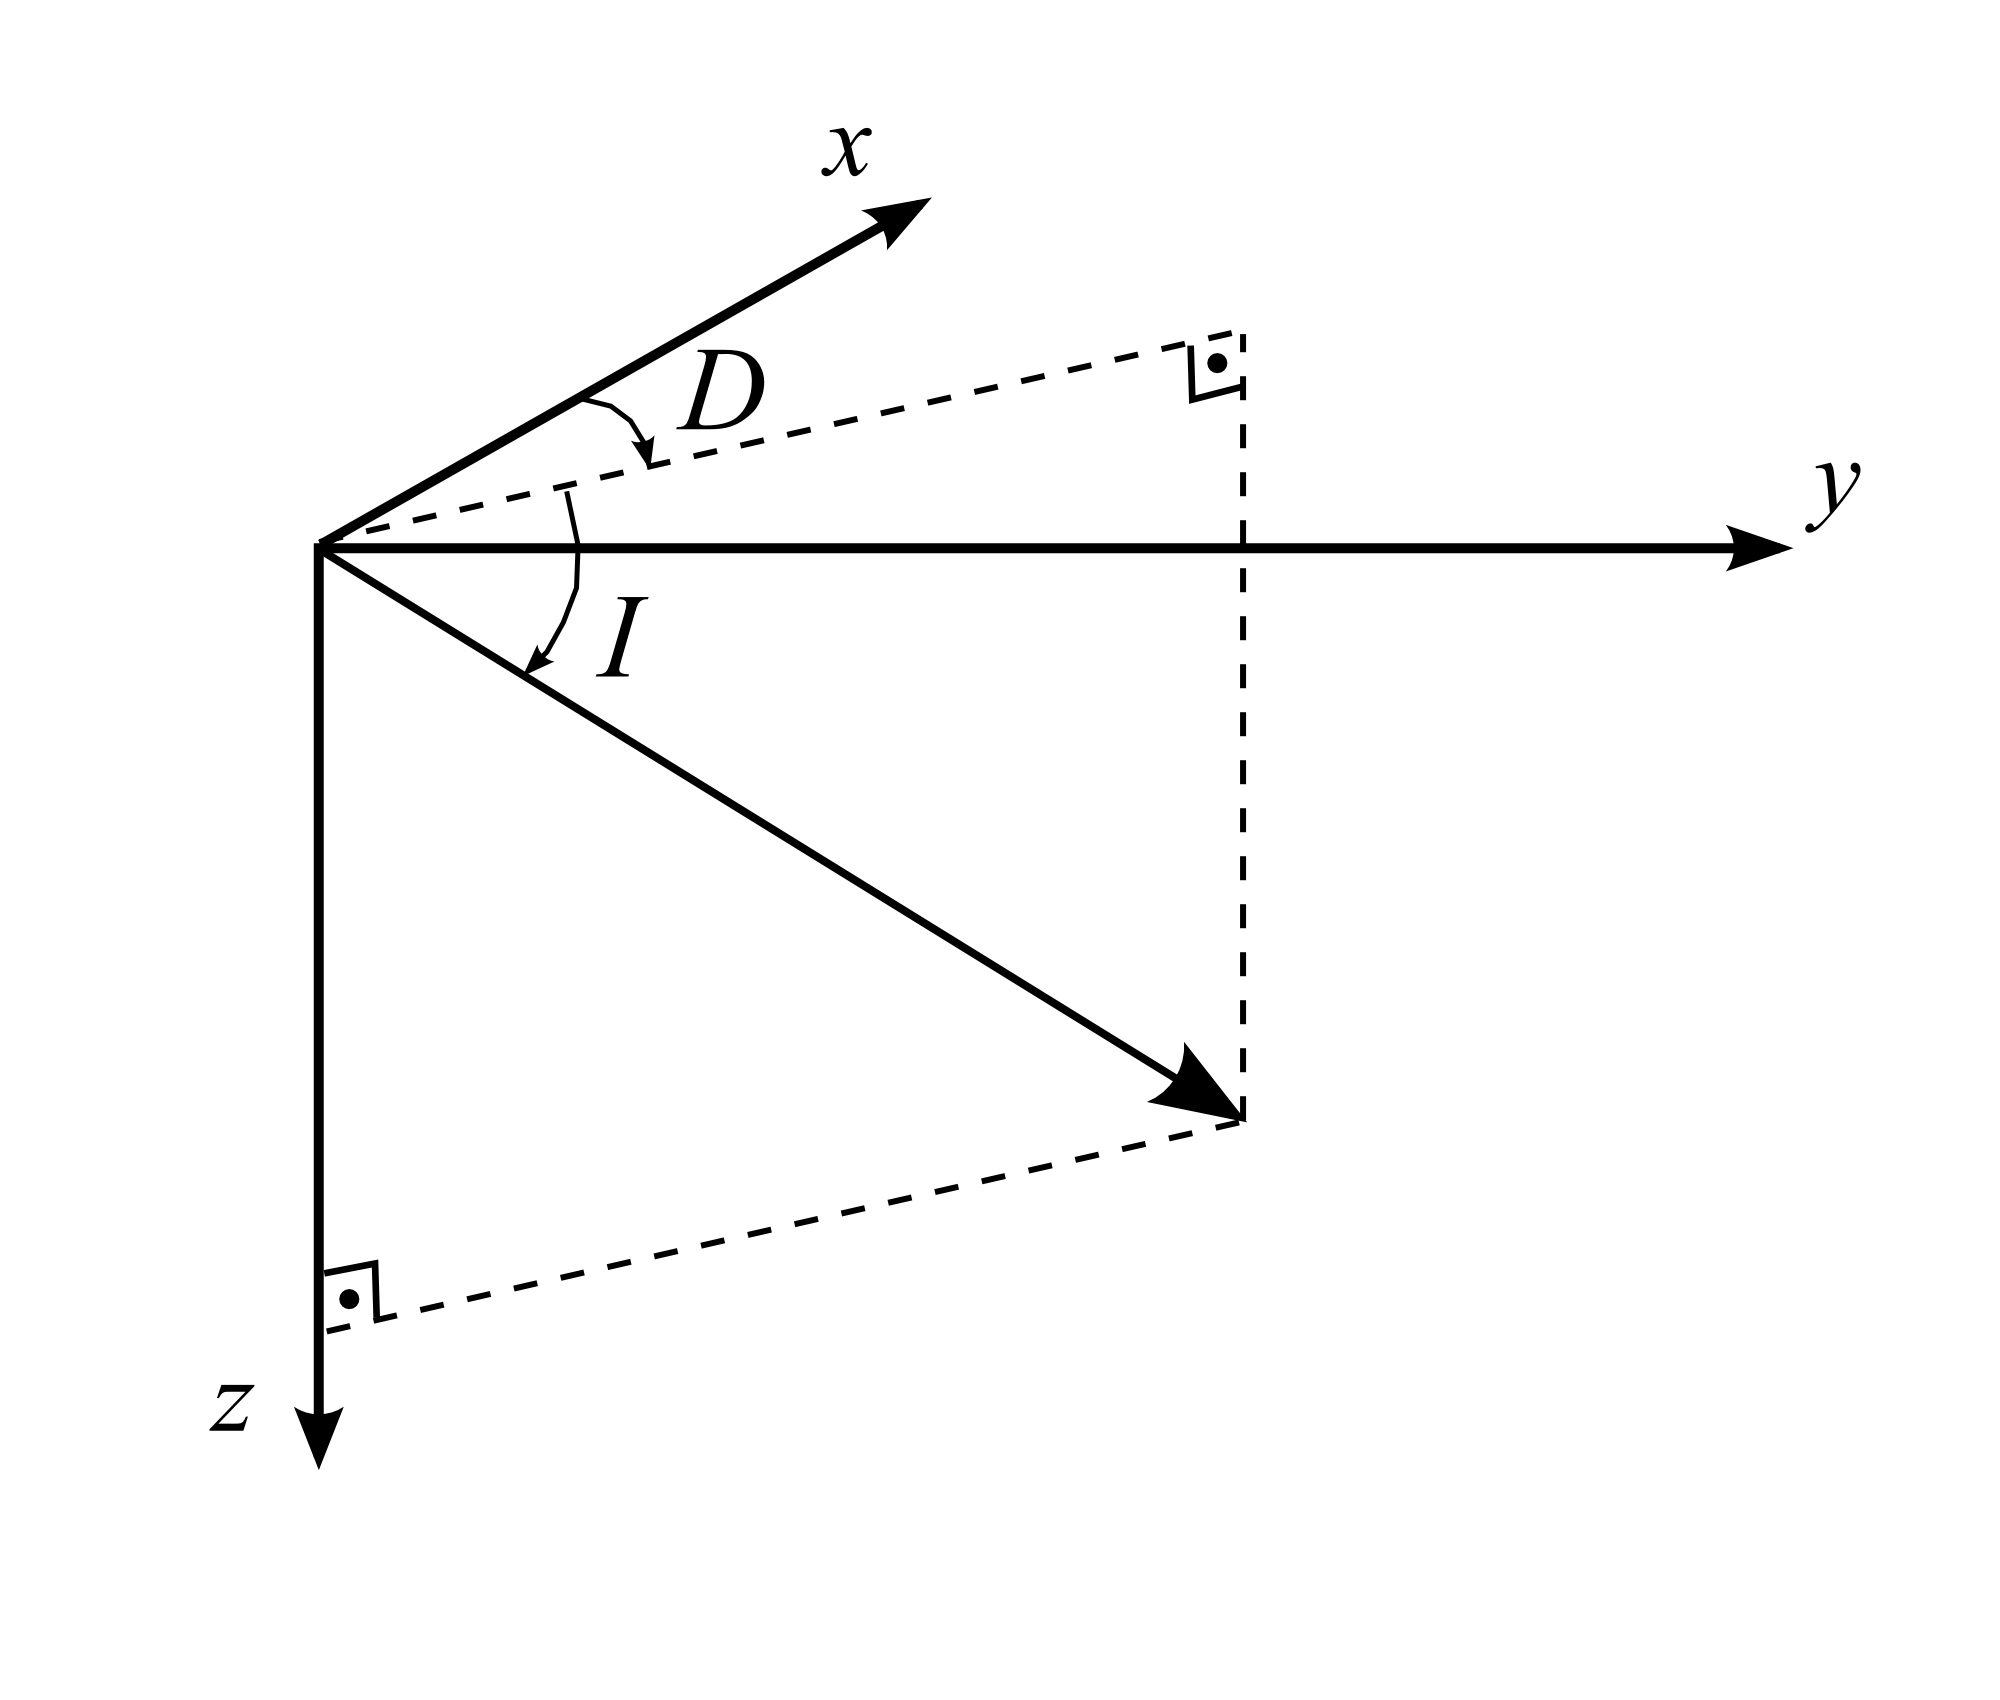
\includegraphics[scale=1]{Fig3.png}
%    \caption{Dist\^{a}ncia $l$ entre um ponto $P$ e outro ponto $P^{\,\prime}$ 
%    de um sistema de coordenadas esféricas.}   
%    \label{fig:fig3}
%\end{figure}
%%<== Figuras
%
\end{document}
